\documentclass[twocolumn,a4j]{jsarticle}
\setlength{\topmargin}{-20.4cm}
\setlength{\oddsidemargin}{-10.4mm}
\setlength{\evensidemargin}{-10.4mm}
\setlength{\textwidth}{18cm}
\setlength{\textheight}{26cm}

\usepackage[top=15truemm,bottom=25truemm,left=15truemm,right=15truemm]{geometry}
\usepackage[latin1]{inputenc}
\usepackage{amsmath}
\usepackage{amsfonts}
\usepackage{amssymb}
\usepackage[dvipdfmx]{graphicx}
\usepackage[dvipdfmx]{color}
\usepackage{listings}
\usepackage{listings,jvlisting}
\usepackage{geometry}
\usepackage{framed}
\usepackage{color}
\usepackage[dvipdfmx]{hyperref}
\usepackage{ascmac}
\usepackage{enumerate}
\usepackage{tabularx}
\usepackage{cancel}
\usepackage{scalefnt}

\renewcommand{\figurename}{Fig.}
\renewcommand{\tablename}{Table }

\lstset{
basicstyle={\ttfamily},
identifierstyle={\small},
commentstyle={\smallitshape},
keywordstyle={\small\bfseries},
ndkeywordstyle={\small},
stringstyle={\small\ttfamily},
frame={tb},
breaklines=true,
columns=[l]{fullflexible},
xrightmargin=0zw,
xleftmargin=3zw,
numberstyle={\scriptsize},
stepnumber=1,
numbersep=1zw,
lineskip=-0.5ex
}

\makeatletter
\def\@maketitle
{
\begin{center}
{\LARGE \@title \par}
\end{center}
\begin{flushright}
{\large 報告書 NO.09 - 1\quad\@date\quad\@author}
\end{flushright}
\par\vskip 1.5em
}
\makeatother

\setcounter{tocdepth}{3}

\author{来代 勝胤}
\title{令和3年度 1月 第1週 報告書}
\date{2022/1/6}

\begin{document}
\columnseprule=0.1mm

\maketitle
\section*{報告内容}
\begin{enumerate}[1.]
    \item 進捗状況
    \item 実験装置の自動化
    \item 実験結果
    \item 補正処理の理論
    \item 校正方法の提案
\end{enumerate}

\section{進捗状況}
自動ステージを用いた実験装置の自動化を目的として実験装置の製作を行った.
また,実験結果の処理方法を検討し,結果として校正実験を行う際に,
その作用力を正しい方向に加えることができれば,ひずみセンサの取付部の状況に関係なく
電圧を作用力へと変換できることがわかった.

\section{実験装置の自動化}
マイクロステージの操作を人為的に行うと
測定時に意図しない電圧変動が起こることや,
操作回数が非常に多くなることから
実験装置の自動化を図った.\\

\subsection{概要}
使用している実験装置にはロードセルを移動させるための地面に対して並行移動するステージと
作用力を与える角度を変化させるための回転ステージが取り付けられている.
この2つのステージを自動ステージヘと換装することで,
実験の効率化とある程度の結果の保証が期待できる.
本実験装置では以下の駿河精機の製品を使用した.

\begin{itemize}
    \item [$\blacksquare$] \textgt{使用した実験装置}
    \item [$\bullet$] 自動ステージコントローラ (DS102)
    \item [$\bullet$] $x$軸マイクロモジュール (PG413-L05AG-C)
    \item [$\bullet$] 自動回転ステージ (KRW06360C-F)
\end{itemize}


\newpage
\section{評価実験}
2021年12月29日(水)から,2022年1月5日(水)にかけて,
製作した実験装置を用いて作用力測定装置の評価実験を行った.\\

\subsection{実験条件}
今回行った実験条件を以下の表1に示す.

\begin{table}[htbp]
    \begin{center}
        \caption{Experimental conditions}
        \begin{tabular}{|p{30mm}|p{20mm}|p{30}|}
            \hline
            \multicolumn{1}{|c|}{\textgt{項目}} & \multicolumn{1}{|c|}{\textgt{条件数}} & \multicolumn{1}{|c|}{\textgt{備考}}\\ \hline
            \multicolumn{1}{|c|}{試験片}                    & \multicolumn{1}{|c|}{1} & \multicolumn{1}{|c|}{\textgt{円筒:実験装置で使用}}  \\ \hline
            \multicolumn{1}{|c|}{測定角度}                    & \multicolumn{1}{|c|}{24} & \multicolumn{1}{|c|}{\textgt{15度ごとの測定}}  \\ \hline
            \multicolumn{1}{|c|}{試行回数}                    & \multicolumn{1}{|c|}{3} & \multicolumn{1}{|c|}{\textgt{}}  \\ \hline
        \end{tabular}
    \end{center}
\end{table}

\subsection{実験方法}
今回の実験では,以前行った模擬実験の方法をもとに検討し,
以下のように設定した.\\

$\blacksquare$ \textgt{測定条件}
    \begin{itemize}
        \item サンプリング周期は5[Hz]とする
        \item ロードセルをマイクロステージを用いて\\
              0.03 [mm] ずつ移動させ,
              作用力を加え電圧を測定する
        \item 基準を0[mm]として,0.03[mm],0.06[mm],0.09[mm],0.12[mm]の計4回移動させる
    \end{itemize}

$\blacksquare$ \textgt{測定準備}
    \begin{enumerate}[(1)]
        \item ロードセルを測定する角度に固定
        \item 粗動用ダイヤルでロードセルを大まかな位置に設定
        \item マイクロステージを動かしてロードセルが供試体に接触する位置を0.01[mm]単位で特定
        \item その位置を基準に測定を開始する
    \end{enumerate}

$\blacksquare$ \textgt{測定方法}
    \begin{enumerate}[(1)]
        \item 測定開始から60秒間待機する
        \item 40秒間の測定時間
        \item 60秒間のマイクロステージ操作時間
        \item (2),(3)の作業を5回繰り返す (100秒周期)\\
              ※ 5回目はロードセル,供試体を非接触状態にする
    \end{enumerate}

\subsection{実験結果}

\newpage

\section{補正処理の理論}
実験を行う過程で,作用力測定装置と回流水槽等の作用力を与える装置を
正しく設置することが非常に困難であることがわかった.
そこで,事前に作用力測定装置のひずみセンサー取付部について,
角度に対する出力電圧の特性を調べ,その結果を用いて,
後に行う校正実験結果に有効的な補正処理方法を検討した.\\

\subsection{校正時の問題点}
校正実験を行い,出力電圧を評価するためには
それぞれの実験装置を正しい方向(角度)に設置する必要がある.
しかし,これまでの実験過程及び結果から,
以下のような要因が校正実験の際に影響を与えていることがわかった.

\begin{itemize}
    \item [$\bullet$] 抗力・揚力方向のひずみセンサが直角に取り付けられていない
    \item [$\bullet$] ひずみセンサ取付部が測定装置の正しく取り付けられていない
    \item [$\bullet$] 実験装置が水流に対して正しい方向に設置されていない
    \item [$\bullet$] 校正装置が正しく取り付けられていない
\end{itemize}

\subsection{座標軸の変換}
ここで,作用力の座標軸について抗力方向を$x軸$,揚力方向を$y$軸,
同様にひずみセンサの座標軸について抗力・揚力方向をそれぞれ$x'$軸,$y'$軸とすると
上記の校正時の問題点により,以下の図のように
ひずみセンサの$x'$軸,$y'$軸は,$x$軸,$y$軸に対して
それぞれ角度$\theta_1$,$\theta_2$だけズレが生じていると考えられる.

\begin{figure}[htbp]
    \footnotesize
    \begin{center}
        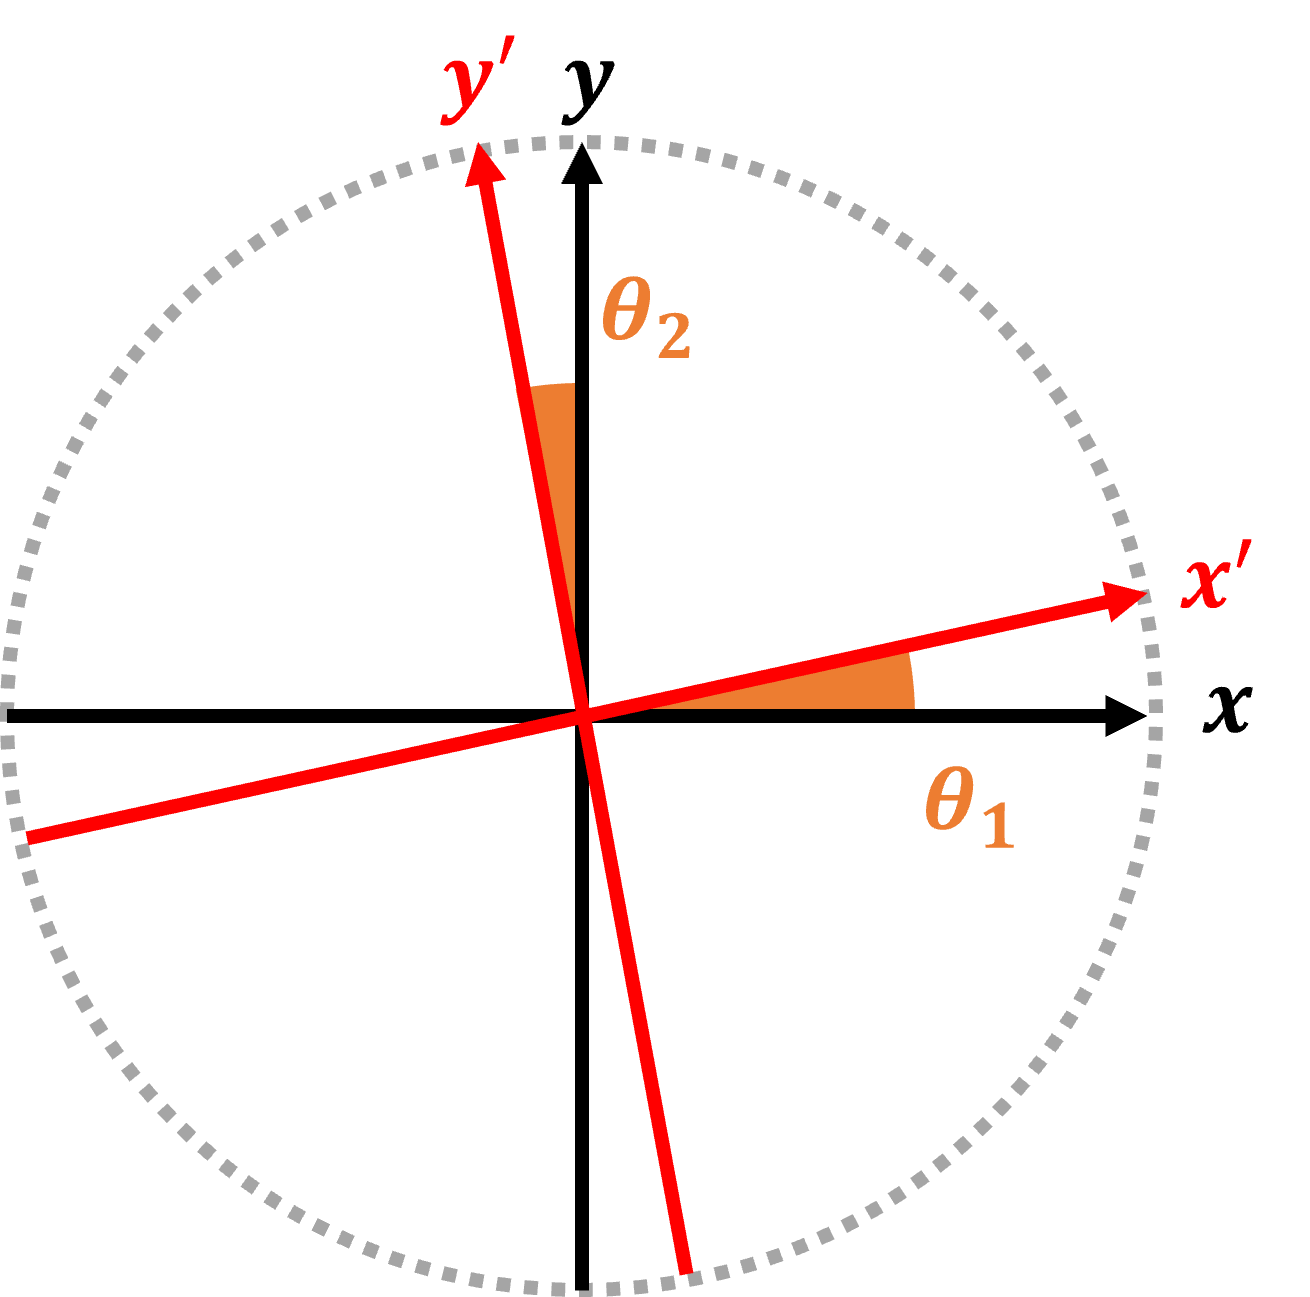
\includegraphics[width=60mm]{../images/image_1.png}
        \caption{theorical Value}
    \end{center}
\end{figure}

このとき,作用力$F$が加えられたとき,以下のような

\section{校正方法の提案}
\end{document}